%*******************************************************************************
%*********************************** First Chapter *****************************
%*******************************************************************************

\chapter{GIỚI THIỆU}  %Title of the First Chapter

\ifpdf
    \graphicspath{{Chapter1/Figs/Raster/}{Chapter1/Figs/PDF/}{Chapter1/Figs/}}
\else
    \graphicspath{{Chapter1/Figs/Vector/}{Chapter1/Figs/}}
\fi


%********************************** %First Section  **************************************
\section{Ý tưởng và tính cấp thiết của đề tài}\label{section1.1}

Ngày nay, bài toán giao thông vẫn đang là bài toán hóc búa vẫn chưa được giải quyết được ở Việt Nam và nhiều nước đang phát triển. Tình trạng kẹt xe, ùn tắc kéo dài gây ra sự chậm trễ trong công việc, hơn nữa còn  gây gia tăng ô nhiễm môi trường, giảm chất lượng môi trường sống. Một trong những khó khăn làm bài toán giao thông khó giải quyết đó chính là không có đầy đủ dữ liệu cần thiết. Chúng ta không thể giải bài toán nếu không có đủ dữ kiện, cũng như giải quyết kẹt xe ta cần phải có dữ liệu về lưu lượng giao thông.

Vì yếu tố trên, dự án SkyNet được hình thành và phát triển theo hướng IoT với mục đích thu thập dữ liệu về các yếu tố môi trường (nồng độ CO, nhiệt độ, chất lượng không khí, độ bụi). Từ đó ta có thể có được 1 phần dữ liệu cần thiết về tình trạng các con đường theo thời gian thực, cũng như có được lịch sử và dùng dữ liệu ấy để phát triển cho những dự án khác.

\begin{figure}[H] 
\centering    
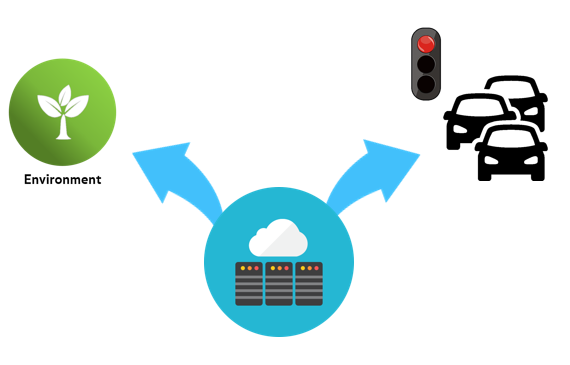
\includegraphics[width=1.0\textwidth]{pic1}
\caption[Mô hình ứng dụng dữ liệu của đề tài]{Mô hình ứng dụng dữ liệu của đề tài}
\label{fig:pic1}
\end{figure}

Và những dữ liệu này có thể ứng dụng cho bất động sản, môi trường và nghiên cứu. Do đó đề tài mang tính thiết thực và ứng dụng cao và được lựa chọn để làm Luận văn tốt nghiệp.


\section{Mục tiêu và nhiệm vụ của đề tài} %Section - 1.1 
\label{section1.2}
\subsection{Mục tiêu đề tài}
\begin{itemize}
\item[-]Tìm hiểu về khí thải xe máy và ô tô.
\item[-]Hiện thực mạch cảm biến để thu thập khí thải.
\item[-]Hiện thực hoàn module thu thập cảm biến tích hợp thêm module sử dụng năng lượng mặt trời để nạp pin cho mạch hoạt động độc lập với điện lưới.
\item[-]Hoàn chỉnh website cho phép người dùng theo dõi thông tin.
\item[-]Đề xuất các tính năng thừa hưởng từ kết quả hệ thống và khả năng tích hợp với các hệ thống khác.
\end{itemize}



\begin{landscape}
\subsection{Nhiệm vụ đề tài}
\begin{table}[]
\centering
\caption{Giản đồ gantt của Huỳnh Phạm So Ny}
\begin{tabular}{|l|l|l|l|l|l|l|l|l|l|l|l|l|l|l|l|l|}
\hline
\multicolumn{1}{|c|}{}                      & \multicolumn{1}{c|}{}                                                                             & \multicolumn{15}{c|}{Tuần}                                                                                                                                                                                                                                                                                                                                                                                                                \\ \cline{3-17} 
\multicolumn{1}{|c|}{\multirow{-2}{*}{STT}} & \multicolumn{1}{c|}{\multirow{-2}{*}{Công việc}}                                                  & 1                        & 2                                               & 3                        & 4                        & 5                        & 6                        & 7                        & 8                        & 9                        & 10                       & 11                       & 12                       & 13                       & 14                       & 15                       \\ \hline
1                                           & \begin{tabular}[c]{@{}l@{}}Tìm hiểu các thiết,bị sensor, MCU, \\ Module SIM\end{tabular}          & \cellcolor[HTML]{000000} & \cellcolor[HTML]{000000}                        & \cellcolor[HTML]{000000} &                          &                          &                          &                          &                          &                          &                          &                          &                          &                          &                          &                          \\ \hline
2                                           & Tìm hiểu về pin,năng lượng mặt trời                                                               &                          & \cellcolor[HTML]{000000}{\color[HTML]{000000} } &                          &                          &                          &                          &                          &                          &                          &                          &                          &                          &                          &                          &                          \\ \hline
3                                           & Làm prototype đầu tiên                                                                            &                          &                                                 &                          & \cellcolor[HTML]{000000} &                          &                          &                          &                          &                          &                          &                          &                          &                          &                          &                          \\ \hline
4                                           & Suy nghĩ design,tổng thể cho cái hộp                                                              &                          &                                                 & \cellcolor[HTML]{000000} & \cellcolor[HTML]{000000} & \cellcolor[HTML]{000000} &                          &                          &                          &                          &                          &                          &                          &                          &                          &                          \\ \hline
5                                           & Thiết kế bản vẽ cho,hộp                                                                           &                          &                                                 &                          &                          &                          & \cellcolor[HTML]{000000} &                          &                          &                          &                          &                          &                          &                          &                          &                          \\ \hline
6                                           & Coding                                                                                            &                          &                                                 &                          &                          &                          & \cellcolor[HTML]{000000} &                          &                          &                          &                          &                          &                          &                          &                          &                          \\ \hline
7                                           & Thiết kế PCB cho,mạch                                                                             &                          &                                                 &                          &                          &                          & \cellcolor[HTML]{000000} & \cellcolor[HTML]{000000} &                          &                          &                          &                          &                          &                          &                          &                          \\ \hline
8                                           & \begin{tabular}[c]{@{}l@{}}Hoàn thiện node cảm biến chạy bằng \\ năng lượng mặt trời\end{tabular} &                          &                                                 &                          &                          &                          &                          & \cellcolor[HTML]{000000} & \cellcolor[HTML]{000000} &                          &                          &                          &                          &                          &                          &                          \\ \hline
9                                           & Testing                                                                                           &                          &                                                 &                          &                          &                          &                          &                          &                          & \cellcolor[HTML]{000000} & \cellcolor[HTML]{000000} & \cellcolor[HTML]{000000} &                          &                          &                          &                          \\ \hline
10                                          & Chọn lại Module SIM và redesign lại PCB                                                           &                          &                                                 &                          &                          &                          &                          &                          &                          &                          &                          & \cellcolor[HTML]{000000} &                          &                          &                          &                          \\ \hline
11                                          & Nhân bản ra 2 node,cảm biến                                                                       &                          &                                                 &                          &                          &                          &                          &                          &                          &                          &                          & \cellcolor[HTML]{000000} & \cellcolor[HTML]{000000} &                          &                          &                          \\ \hline
12                                          & Đi thu thập dữ liệu  \& viết báo cáo                                                              &                          &                                                 &                          &                          &                          &                          &                          &                          &                          &                          &                          &                          & \cellcolor[HTML]{000000} & \cellcolor[HTML]{000000} & \cellcolor[HTML]{000000} \\ \hline
\end{tabular}
\end{table}
\end{landscape}











\begin{landscape}

\begin{table}[]
\centering
\caption{Giản đồ gantt của Nguyễn Mạnh Cường}
\begin{tabular}{|l|l|l|l|l|l|l|l|l|l|l|l|l|l|l|l|l|}
\hline
\multicolumn{1}{|c|}{}                      & \multicolumn{1}{c|}{}                                                                                                 & \multicolumn{15}{c|}{Tuần}                                                                                                                                                                                                                                                                                                                                                                                         \\ \cline{3-17} 
\multicolumn{1}{|c|}{\multirow{-2}{*}{STT}} & \multicolumn{1}{c|}{\multirow{-2}{*}{Công việc}}                                                                      & 1                        & 2                        & 3                        & 4                        & 5                        & 6                        & 7                        & 8                        & 9                        & 10                       & 11                       & 12                       & 13                       & 14                       & 15                       \\ \hline
1                                           & \begin{tabular}[c]{@{}l@{}}Tìm hiểu về web,server, Nodejs, \\ mô hình template cho web\end{tabular}                   & \cellcolor[HTML]{000000} & \cellcolor[HTML]{000000} &                          &                          &                          &                          &                          &                          &                          &                          &                          &                          &                          &                          &                          \\ \hline
2                                           & \begin{tabular}[c]{@{}l@{}}Tìm hiểu high,chart, Json cho \\ việc hiện thực biểu đồ\end{tabular}                       &                          &                          & \cellcolor[HTML]{000000} & \cellcolor[HTML]{000000} &                          &                          &                          &                          &                          &                          &                          &                          &                          &                          &                          \\ \hline
3                                           & \begin{tabular}[c]{@{}l@{}}Hiện thực các chức,năng cho server\\ (google map, add,config Node, graph...)\end{tabular}  &                          &                          &                          & \cellcolor[HTML]{000000} & \cellcolor[HTML]{000000} & \cellcolor[HTML]{000000} & \cellcolor[HTML]{000000} &                          &                          &                          &                          &                          &                          &                          &                          \\ \hline
4                                           & Tìm hiểu về Node,Mailer, hiện thựcsend mail                                                                           &                          &                          &                          &                          &                          &                          & \cellcolor[HTML]{000000} & \cellcolor[HTML]{000000} &                          &                          &                          &                          &                          &                          &                          \\ \hline
5                                           & Tìm hiểu Ionic,framework                                                                                              &                          &                          &                          &                          &                          &                          &                          &                          & \cellcolor[HTML]{000000} & \cellcolor[HTML]{000000} &                          &                          &                          &                          &                          \\ \hline
6                                           & \begin{tabular}[c]{@{}l@{}}Hiện thực giao diện mobile app và \\ một số chức năng, tìm hiểu angular chart\end{tabular} &                          &                          &                          &                          &                          &                          &                          &                          &                          & \cellcolor[HTML]{000000} & \cellcolor[HTML]{000000} & \cellcolor[HTML]{000000} &                          &                          &                          \\ \hline
7                                           & \begin{tabular}[c]{@{}l@{}}Hoàn thiện web,server, sửa lỗi một số \\ chức năng \& viết báo cáo\end{tabular}            &                          &                          &                          &                          &                          &                          &                          &                          &                          &                          &                          &                          & \cellcolor[HTML]{000000} & \cellcolor[HTML]{000000} & \cellcolor[HTML]{000000} \\ \hline
\end{tabular}
\end{table}

\end{landscape}



\begin{landscape}
\begin{table}[]
\centering
\caption{Giản đồ gantt của Võ Tấn Tùng}
\begin{tabular}{|l|l|l|l|l|l|l|l|l|l|l|l|l|l|l|l|l|}
\hline
\multicolumn{1}{|c|}{}                      & \multicolumn{1}{c|}{}                                                                                            & \multicolumn{15}{c|}{Tuần}                                                                                                                                                                                                                                                                                                                                                                                                                                                              \\ \cline{3-17} 
\multicolumn{1}{|c|}{\multirow{-2}{*}{STT}} & \multicolumn{1}{c|}{\multirow{-2}{*}{Công việc}}                                                                 & 1                        & 2                                               & 3                        & 4                        & 5                        & 6                        & 7                                               & 8                        & 9                        & 10                                              & 11                       & 12                       & 13                       & 14                       & 15                       \\ \hline
1                                           & Tìm hiểu về các công cụ hỗ trợ xây dựng server                                                                   & \cellcolor[HTML]{000000} & \cellcolor[HTML]{000000}                        &                          &                          &                          &                          &                                                 &                          &                          &                                                 &                          &                          &                          &                          &                          \\ \hline
2                                           & Tìm hiểu về các công cụ lập trình web                                                                            &                          & \cellcolor[HTML]{000000}{\color[HTML]{FFFFFF} } &                          &                          &                          &                          &                                                 &                          &                          &                                                 &                          &                          &                          &                          &                          \\ \hline
3                                           & Tìm hiểu và lựa chọn Database phù hợp                                                                            &                          & \cellcolor[HTML]{000000}                        & \cellcolor[HTML]{000000} &                          &                          &                          &                                                 &                          &                          &                                                 &                          &                          &                          &                          &                          \\ \hline
4                                           & Thiết kế mô hình hệ thống server                                                                                 &                          &                                                 &                          & \cellcolor[HTML]{000000} & \cellcolor[HTML]{000000} &                          &                                                 &                          &                          &                                                 &                          &                          &                          &                          &                          \\ \hline
5                                           & Khởi tạo Server và Database server                                                                               &                          &                                                 &                          &                          & \cellcolor[HTML]{000000} &                          &                                                 &                          &                          &                                                 &                          &                          &                          &                          &                          \\ \hline
6                                           & Thiết kế APIs và Server URL Routing                                                                              &                          &                                                 &                          &                          &                          & \cellcolor[HTML]{000000} &                                                 &                          &                          &                                                 &                          &                          &                          &                          &                          \\ \hline
7                                           & Hiện thực APIs                                                                                                   &                          &                                                 &                          &                          &                          & \cellcolor[HTML]{000000} & \cellcolor[HTML]{000000}                        &                          &                          &                                                 &                          &                          &                          &                          &                          \\ \hline
8                                           & \begin{tabular}[c]{@{}l@{}}Thử nghiệm tính ổn định APIs \\ với mạch sensor node\end{tabular}                     &                          &                                                 &                          &                          &                          &                          & \cellcolor[HTML]{000000}{\color[HTML]{000000} } &                          &                          &                                                 &                          &                          &                          &                          &                          \\ \hline
9                                           & \begin{tabular}[c]{@{}l@{}}Hiện thực URL Web Routing và nhúng\\ code frontend\end{tabular}                       &                          &                                                 &                          &                          &                          &                          & \cellcolor[HTML]{000000}                        & \cellcolor[HTML]{000000} & \cellcolor[HTML]{000000} &                                                 &                          &                          &                          &                          &                          \\ \hline
10                                          & \begin{tabular}[c]{@{}l@{}}Tìm hiểu và khởi tạo Server chạy \\ trên Raspberry\end{tabular}                       &                          &                                                 &                          &                          &                          &                          &                                                 & \cellcolor[HTML]{000000} &                          &                                                 &                          &                          &                          &                          &                          \\ \hline
11                                          & \begin{tabular}[c]{@{}l@{}}Duyệt lại và chỉnh sửa các đoạn code \\ xung đột và tối ưu code frontend\end{tabular} &                          &                                                 &                          &                          &                          &                          &                                                 &                          & \cellcolor[HTML]{000000} & \cellcolor[HTML]{000000}                        &                          &                          &                          &                          &                          \\ \hline
12                                          & Hiện thực xác thực người dùng                                                                                    &                          &                                                 &                          &                          &                          &                          &                                                 &                          &                          & \cellcolor[HTML]{000000}{\color[HTML]{000000} } & \cellcolor[HTML]{000000} &                          &                          &                          &                          \\ \hline
13                                          & \begin{tabular}[c]{@{}l@{}}Hiện thực cung cấp log và trang log \\ cho nhà phát triển\end{tabular}                &                          &                                                 &                          &                          &                          &                          &                                                 &                          &                          &                                                 & \cellcolor[HTML]{000000} &                          &                          &                          &                          \\ \hline
14                                          & Hiện thực trang thống kê statis                                                                                  &                          &                                                 &                          &                          &                          &                          &                                                 &                          &                          &                                                 &                          & \cellcolor[HTML]{000000} &                          &                          &                          \\ \hline
15                                          & Duyệt và tối ưu hóa code Server                                                                                  &                          &                                                 &                          &                          &                          &                          &                                                 &                          &                          &                                                 &                          & \cellcolor[HTML]{000000} & \cellcolor[HTML]{000000} &                          &                          \\ \hline
16                                          & Đánh giá hệ thống và viết báo cáo                                                                                &                          &                                                 &                          &                          &                          &                          &                                                 &                          &                          &                                                 &                          &                          & \cellcolor[HTML]{000000} & \cellcolor[HTML]{000000} & \cellcolor[HTML]{000000} \\ \hline
\end{tabular}
\end{table}
\end{landscape}


\section{Cấu trúc báo cáo} %Section - 1.1 
Luận văn được chia thành 5 chương, nội dung chính của mỗi chương như sau:

\textbf{Chương 1: Giới thiệu}\\
Giới thiệu sơ bộ về ý tưởng cũng như tính cấp bách, mục tiêu và nhiệm vụ của đề tài và cấu trúc bản báo cáo.

\textbf{Chương 2: Cơ sở lý thuyết}\\
Giới thiệu lý thuyết về các yếu tố ảnh hưởng tới chất lượng môi trường và các hệ thống quan trắc hiện hữu. Bên cạnh đó trình bày kiến thức nền tảng về Internet of Things, các công cụ và thiết bị phần cứng hỗ trợ phát triển IoT được áp dụng thực hiện đề tài. Bên cạnh đó là các khái niệm về các công nghệ, nền tảng xây dựng Server và Database được sử dụng cũng như phát triển ứng dung web và di động cụ thể của hệ thống.

\textbf{Chương 3: Thiết kế}\\
Chương này trình bày thiết kế, cách thức hoạt động của hệ thống, các loại cảm biến được sử dụng và chuẩn giao tiếp được sử dụng.

\textbf{Chương 4: Hiện thực và thử nghiệm}\\
Hiện thực dựa trên bản thiết kế được trình bày, hiện thực các sensor node, hệ thống Server , ứng dụng Web và di động.

Sau khi hiện thực, nhóm thống kê những kết quả thực tế đo được, đánh giá mức độ ổn định của sensor node và server cũng như trải nghiệm ứng dụng web và di động.

\textbf{Chương 5: Tổng kết}\\
Chương này sẽ đút kết những gì đạt được và khó khăn trong việc hiện thực đề tài. Bên cạnh đó đề ra hướng phát triển đề tài trong tương lai.

